\theoremstyle{definition}
\newtheorem{defn}{Definition}
\theoremstyle{plain}
\newtheorem{thm}{Theorem}
\theoremstyle{plain}
\newtheorem{lem}[thm]{Lemma}

\def\defnautorefname~#1\null{%
  Definition~(#1)\null
}
\def\thmautorefname~#1\null{%
  Theorem~(#1)\null
}
\def\lemautorefname~#1\null{%
  Lemma~(#1)\null
}

\section{Formalisation in Type Theory}
\par Let us recall the two components of our formalisation: the
translation of regular expressions to DFA and the correctness proofs
of the translation. The translation is
divided into several steps. Firstly, any regular expression is
converted into an \(\epsilon\)-NFA using Thompson's construction
\cite{thompson1968}. Secondly, all the \(\epsilon\)-transitions are
removed by computing the \(\epsilon\)-closures. Thirdly, a DFA is built by using powerset
construction. After that, all the unreachable
states are removed. Finally, a minimal DFA is obtained by using
quotient construction. The translation is correct if and only if 1) the
accepting languages of the regular expression and its translated
output are equal, i.e. \(L(regex) = L(\)translated \(\epsilon\)-NFA\() = L(\)translated DFA\() =
L(\)translated MDFA\()\) and 2) the translated MDFA is minimal. 

\par In this section, we will walk through the formalisation of
each of the above steps and their correctness proofs. Note
that all the definitions, theorems, lemmas and proofs written in this section
are adapted to the environment of Agda. Now let us begin with the 
representation of subsets and languages. 


\subsection{Subsets and Decidable Subsets}
\par The types of subsets and decidable subsets are defined in
\textbf{Subset.agda} and \textbf{Subset/DecidableSubset.agda}
respectively along with their operations such as membership (\(\in\)), subset
(\(\subseteq\)), superset (\(\supseteq\)) and equality (\(=\)). Let us
begin with the definition of general subsets. To separate the
operations of subsets and decidable subsets, all the operations of
decidable subset are denoted by the superscript (\(^d\)), e.g. \(\in^d\)
is the membership decider for decidable subsets. 

\begin{defn} 
\noindent Suppose \(A\) is a set, then its
subsets are represented as unary functions on
\(A\) in Type Theory, i.e. \(Subset\ A = A \to Set\). 
\end{defn}

\par In our definition, a subset is a function from \(A\) to
\(Set\). When declaring a subset, we can write \(sub =
\lambda\ (x : A) \to\ P\ x\). \(P\ x\) defines the conditions for \(x\) to
be included in \(sub\). This construction is
very similar to set comprehension. For example, the above subset
corresponds to \(\{x\ | \ x \in A,\ P(x)\}\). Furthermore, \(sub\) is
also a predicate on \(A\) as its type is in the form of \(A \to
Set\) and its decidability will remain unknown until it is either proved or disproved. 

\begin{defn} 
\noindent Another representation of subset is \(DecSubset\ A = A \to
Bool\). Unlike \(Subset\), its decidability is ensured by its
definition. 
\end{defn}

\par The two representations have different roles in the project. For
example, \(Language\) is defined using \(Subset\) as not every
language is decidable. For other parts in the project 
such as the subsets of states in an automaton, \(DecSubset\) is used
because the decidability is assumed. 


\subsection{Languages}
\par The type of languages is defined in \textbf{Language.agda} along with its 
operations and lemmas such as union (\(\cup\)), concatenation
(\(\bullet\)) and closure (\(\star\)). 

\par We represent the set of alphabets \(\Sigma\) as a data type in
Type Theory, i.e. \(\Sigma : Set\). Note that the equality relation of \(\Sigma\) needs to be
decidable. In Agda, they are passed to every module as
parameters, e.g. \(module\ Language (\Sigma : Set)\ (dec : DecEq\
\Sigma)\ where\). 

\begin{defn}
\noindent We first define \(\Sigma^*\) as the set of all
strings over \(\Sigma\). In our approach, it is expressed as a list of
alphabets, i.e. \(\Sigma^* = List\ \Sigma\). 
\end{defn}

\par For example, (\(A :: g :: d :: a :: [\ ]\)) is equivalent to the
string 'Agda' and the empty list \([\ ]\)
represents the empty string (\(\epsilon\)). In this way, the first
alphabet can be extracted from the input string by pattern matching in order to
run a transition from a particular state to another state in an automaton. 

\begin{defn}
\noindent A language is defined as a subset of 
\(\Sigma^*\), i.e. \(Language = Subset\ \Sigma^*\). 
Note that \(Subset\) instead of \(DecSubset\) is used because not
every language is decidable. 
\end{defn}

\subsubsection{Operations on Languages}

\begin{defn} 
\label{defn:lang_union}
\noindent Suppose \(L_1\) and \(L_2\) are languages, then the union of
the two languages, \(L_1\cup L_2\), is given by the set \(\{w\
|\  w \in L_1\ \vee \ w \in L_2\}\). In Type Theory, we have \(L_1 \cup L_2 = \lambda\ w
\to w \in L_1\ \uplus\ w \in L_2\).
\end{defn}

\begin{defn}
\label{defn:lang_con}
\noindent Suppose \(L_1\) and \(L_2\) are languages, then
the concatenation of the two languages, \(L_1\bullet L_2\), is given
by the set \(\{w\  |\  \exists u\in L_1.\ \exists v\in L_2.\ w = uv\}\). In
Type Theory, we have \(L_1\bullet L_2 = \lambda\ w \to \exists[\
u \in \Sigma^*\ ]\ \exists[\ v \in \Sigma^*\ ] (u \in L_1 \times v \in
L_2 \times w \equiv u\ \Plus\Plus\  v )\).
\end{defn}

\begin{defn}
\label{defn:lang_power}
\noindent Suppose \(L\) is a language, then we define \(L^n\) as
the concatenation of \(L\) with itself over \(n\) times, i.e. \(L^n =
L\bullet L\bullet L ... L\). In Type Theory, it is defined as a recursive function where \(L \wedge zero = [\![\epsilon ]\!]\) and
\(L \wedge (suc\ n) = L \bullet (L \wedge n)\). 
\end{defn}

\begin{defn}
\label{defn:lang_star}
\noindent Suppose \(L\) is a language, then the closure of
L, \(L\ast\) is given by the set \(\bigcup_{n \in N} L^n\). In Type
Theory, we have \(L\ \star = \lambda\ w \to \exists [\ n \in \mathbb{N}\
]\ (w \in L \wedge n)\). 
\end{defn}


\subsection{Regular Expressions and Regular Languages}
\par The types of regular expressions and regular languages are defined in
\textbf{RegularExpression.agda}. 

\begin{defn}
\label{defn:regex}
\noindent Regular expressions over \(\Sigma\) are defined inductively as follow: 
\begin{enumerate}[nolistsep]
  \item \(\O\) is a regular expression denoting the regular language \(\O\);
  \item \(\epsilon\) is a regular expression denoting the regular language \(\{\epsilon\}\);
  \item \(\forall a\in\Sigma.\ a\) is a regular expression denoting the regular language \(\{a\}\);
  \item if \(e_{1}\) and \(e_{2}\) are regular expressions denoting the regular
    languages \(L_1\) and \(L_2\) respectively, then
    \begin{enumerate}[nolistsep]
      \item \(e_{1}\ |\ e_{2}\) is a regular expressions denoting the
        regular language \(L_1 \cup L_2\);
      \item \(e_{1}\cdot e_{2}\) is a regular expression denoting the
        regular language \(L_1\bullet L_2\);
      \item \(e_{1}^{\ *}\) is a regular expression denoting the regular
        language \(L_1\ \star\).
     \end{enumerate}
\end{enumerate}
\end{defn}

\par The interpretation of regular expression in Agda is as follow:

\begin{lstlisting}[mathescape=true,xleftmargin=.3\textwidth]
data RegExp : Set where
  $\O$    : RegExp
  $\epsilon$    : RegExp
  $\sigma$    : $\Sigma$ $\to$ RegExp
  _|_ : RegExp $\to$ RegExp $\to$ RegExp
  _$\cdot$_  : RegExp $\to$ RegExp $\to$ RegExp
  _$^*$  : RegExp $\to$ RegExp
\end{lstlisting} 

\par The accepting language of regular expressions is defined as
a function from \(RegExp\) to \(Language\). 

\begin{lstlisting}[mathescape=true,xleftmargin=.3\textwidth]
L$^R$ : RegExp $\to$ Language
L$^R$ $\O$   = $\o$
L$^R$ $\epsilon$   = $[\![\epsilon ]\!]$
L$^R$ ($\sigma$ a) = $[\![\ a\ ]\!]$
L$^R$ (e$_1$ | e$_2$) = L$^R$ e$_1$ $\cup$ L$^R$ e$_2$
L$^R$ (e$_1$ $\cdot$ e$_2$) = L$^R$ e$_1$ $\bullet$ L$^R$ e$_2$
L$^R$ (e$^*$) = (L$^R$ e) $\star$
\end{lstlisting} 


\subsection{\(\epsilon\)-Non-deterministic Finite Automata}
\par Recall that the set of all strings over \(\Sigma\) is defined as
the type \(List\ \Sigma^*\). However, this definition gives us no way to
extract an \(\epsilon\) alphabet from the input string. Therefore,
we need to introduce another representation specific to this purpose. 

\begin{defn}
\noindent We define \(\Sigma^e\) as the union of
\(\Sigma\) and \(\{\epsilon\}\), i.e. \(\Sigma^e = \Sigma \cup \{\epsilon\}\).
\end{defn} 

\par The equivalent data type is as follow:
\begin{lstlisting}[mathescape=true,xleftmargin=.3\textwidth]
data $\Sigma^e$ : Set where
  $\alpha$ : $\Sigma \to \Sigma^e$
  E : $\Sigma^e$
\end{lstlisting}

\par All the alphabets in \(\Sigma\) are included in \(\Sigma^e\) by using the
\(\alpha\) constructor while the \(\epsilon\) alphabet corresponds to
the constructor \(E\) in the data type. 

\begin{defn}
\noindent Now we define \(\Sigma^{e*}\), the set of all strings over
\(\Sigma^e\) in a way similar to \(\Sigma^*\), i.e. \(\Sigma^{e*} =
List\ \Sigma^e\). 
\end{defn}

\par For example, the string 'Agda' can be
represented by (\(\alpha\ A :: \alpha\ g :: E :: \alpha\ d :: E :: \alpha\
a :: [\ ]\)) or (\(E :: \alpha\ A :: E :: E :: \alpha\ g :: \alpha\ d ::
E :: \alpha\ a :: [\ ]\)). We call these two lists as the \(\epsilon\)-strings of the
string 'Agda'. All the definitions, operations and lemmas regarding
\(\epsilon\)-strings can be found in \textbf{Language.agda}. 

\par Now, let us define \(\epsilon\)-NFA using \(\Sigma^{e*}\). The
type of \(\epsilon\)-NFA is defined in \textbf{eNFA.agda} along with its operations and
properties. 

\begin{defn}
\noindent An \(\epsilon\)-NFA is a 5-tuple \(M = (Q
,\ \Sigma^e,\ \delta,\ q_0,\ F)\), where
\begin{enumerate}[nolistsep]
  \item \(Q\) is a finite set of states;
  \item \(\Sigma^e\) is the union of \(\Sigma\) and \(\{\epsilon\}\);
  \item \(\delta\) is a mapping from \(Q \times \Sigma^e\) to
    \(\mathcal P \left({Q}\right)\) that defines the behaviour of the automata;
  \item \(q_0\) in \(Q\) is the initial state;
  \item \(F \subseteq Q\) is the set of accepting states. 
\end{enumerate}
\end{defn}

\par It is formalised as a record in Agda as shown below: 

\begin{lstlisting}[mathescape=true,xleftmargin=.3\textwidth]
record $\epsilon \hyphen$NFA : Set$_1$ where
  field
    Q      : Set
    $\delta$       : Q $\to$ $\Sigma^e$ $\to$ DecSubset Q
    q$_0$      : Q
    F      : DecSubset Q
    $\forall$qEq    : $\forall$ q $\to$ q $\in^d$ $\delta$ q E
    Q?     : DecEq Q
    |Q|-1  : $\mathbb{N}$
    It     : Vec Q (suc |Q|-1)
    $\forall$q$\in$It    : (q : Q) $\to$ (q $\in^V$ It)
    unique : Unique It
\end{lstlisting}

\par The set of alphabets \(\Sigma\) is passed into the module as a
parameter and \(\Sigma^e\) is constructed using \(Sigma\). Together with \(Q\), \(\delta\),
\(q_0\) and \(F\), these five fields correspond to the 5-tuple
\(\epsilon\)-NFA. The other extra fields are used when computing
\(\epsilon\)-closures. They are \(\forall qEq\) -- a proof that any
state in \(Q\) can reach itself by an
\(\epsilon\)-transition; \(Q?\) -- the decidable equality of \(Q\);
\(|Q|-1\) -- the number of states minus 1; \(It\) -- a vector of
containing all the states in \(Q\); \(\forall q\in It\)
-- a proof that every state in \(Q\) is also in the vector
\(It\); and \(unique\) -- a proof that there is no repeating elements in
\(It\). 

\par Now, before we can define the accepting language of a given
\(\epsilon\)-NFA, we need to define several operations of
\(\epsilon\)-NFA. 

\begin{defn}
\noindent A configuration is composed of a state and an alphabet from
\(\Sigma^e\), i.e. \(C = Q \times \Sigma^e\). 
\end{defn}

\begin{defn}
\noindent A move in an \(\epsilon\)-NFA \(N\) is
represented by a binary function (\(\vdash\)) on two configurations. We say
that for all \(w \in \Sigma^{e*}\) and \(a \in \Sigma^e\), \((q, aw)
\vdash (q' , w)\) if and only if \(q' \in \delta (q , a)\). 
\end{defn}

\par The binary function is defined in Agda as follow: 
\begin{lstlisting}[mathescape=true,xleftmargin=.3\textwidth]
  _$\vdash$_ : (Q $\times$ $\Sigma^e$ $\times$ $\Sigma^{e*}$) $\to$ (Q $\times$ $\Sigma^{e*}$) $\to$ Set
  (q , a , w) $\vdash$ (q' , w') = w $\equiv$ w' $\times$ q' $\in^d$ $\delta$ q a
\end{lstlisting}

\begin{defn}
\noindent Suppose \(C\) and \(C'\) are configurations. We say that \(C \vdash^0 C'\) if and only
if \(C = C'\); and \(C_0 \vdash^k C_k\) for any \(k \geq 1\) if and only if there exists a chain of
configurations \(C_1, C_2, ..., C_{k-1}\) such that \(C_i \vdash C_{i+1}\) for all \(0 \leq i < k\). 
\end{defn}

\par It is defined as a recursive function in Agda as follow: 
\begin{lstlisting}[mathescape=true,xleftmargin=.3\textwidth]
  _$\vdash^k$_-_ : (Q $\times$ $\Sigma^{e*}$) $\to$ $\mathbb{N}$ $\to$ (Q $\times$ $\Sigma^{e*}$) $\to$ Set
  (q , w$^e$) $\vdash^k$ zero  - (q' , w$^e$')
    = q $\equiv$ q' $\times$ w$^e$ $\equiv$ w$^e$'
  (q , w$^e$) $\vdash^k$ suc n - (q' , w$^e$') 
    = $\exists$[ p $\in$ Q ] $\exists$[ a$^e$ $\in$ $\Sigma^e$ ] $\exists$[ u$^e$ $\in$ $\Sigma^{e*}$ ]
      (w$^e$ $\equiv$ a$^e$ :: u$^e$ $\times$ (q , a$^e$ , u$^e$) $\vdash$ (p , u$^e$) $\times$ (p , u$^e$) $\vdash^k$ n - (q' , w$^e$'))
\end{lstlisting}

\begin{defn}
\noindent We say that \(C \vdash^* C'\) if and only
if there exists a number of chains \(n\) such that \(C \vdash^n C'\). 
\end{defn}

\par Its corresponding type is defined as follow: 
\begin{lstlisting}[mathescape=true,xleftmargin=.3\textwidth]
  _$\vdash^*$_ : (Q $\times$ $\Sigma^{e*}$) $\to$ (Q $\times$ $\Sigma^{e*}$) $\to$ Set
  (q , w$^e$) $\vdash^*$ (q' , w$^e$') = $\exists$[ n $\in$ $\mathbb{N}$ ] (q , w$^e$) $\vdash^k$ n - (q' , w$^e$')
\end{lstlisting}

\begin{defn}
\label{defn:enfa}
\noindent For any string \(w\), it is accepted by an \(\epsilon\)-NFA
if and only if there exists an \(\epsilon\)-string of \(w\)
that can take \(q_0\) to an accepting state \(q\). Therefore, the
accepting language of an \(\epsilon\)-NFA is given by the set \(\{\ w\ |\ \exists w^e\in
\Sigma^{e*}.\ w = to\Sigma^*(w^e) \wedge \exists q\in F.\ (q_0,w^e) \vdash^* (q,\epsilon)\ \}\). 
\end{defn}

\par The corresponding formalisation in Agda is as follow: 
\begin{lstlisting}[mathescape=true,xleftmargin=.3\textwidth]
  L$^{eN}$ : $\epsilon \hyphen$NFA $\to$ Language
  L$^{eN}$ nfa = $\lambda$ w $\to$ 
            $\exists$[ w$^e$ $\in$ $\Sigma^{e*}$ ] (w $\equiv$ $to\Sigma^*$ w$^e$ $\times$ ($\exists$[ q $\in$ Q ] (q $\in^d$ F $\times$ (q$_0$ , w$^e$) $\vdash^*$ (q , []))))
\end{lstlisting} 


\subsection{Thompson's Construction}
\par Now, let us look at the translation of regular expressions to
\(\epsilon\)-NFA which is defined in \textbf{Translation/RegExp-eNFA.agda}. 

\begin{defn}
\label{defn:thompson}
\noindent The translation of regular expressions
to \(\epsilon\)-NFA is defined inductively as follow:
\begin{enumerate}[nolistsep]
  \item for \(\O\), we have \(M = (\{init\},\ \Sigma^e,\ \delta,\
    init,\ \O)\) and graphically \begin{center}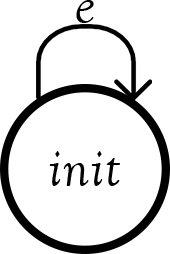
\includegraphics{null}\end{center}
  \item for \(\epsilon\), we have \(M = (\{init\},\ \Sigma^e,\
    \delta,\ init,\ \{init\})\) and graphically \begin{center}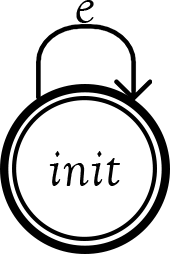
\includegraphics{epsilon}\end{center}
  \item for \(a\), we have \(M = (\{init, accept\},\ \Sigma^e,\
    \delta,\ init,\ \{accept\})\) and graphically \begin{center}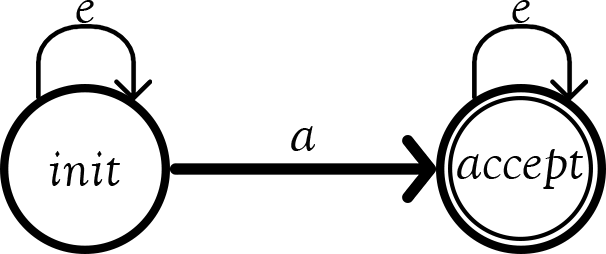
\includegraphics{singleton}\end{center}
  \item suppose \(N_1 = (Q_1,\ \delta_1,\ q_{01},\ F_1)\) and \(N_2 =
    (Q_2,\ \delta_2,\ q_{02},\ F_2)\) are \(\epsilon\)-NFAs translated from the
    regular expressions \(e_1\) and \(e_2\) respectively, then
    \begin{enumerate}[nolistsep]
      \item for \((e_1\ |\ e_2)\), we have \(M = (\{init\} \cup Q_1
        \cup Q_2,\ \Sigma^e,\ \delta,\ init,\ F_1 \cup F_2)\) and
        graphically \begin{center}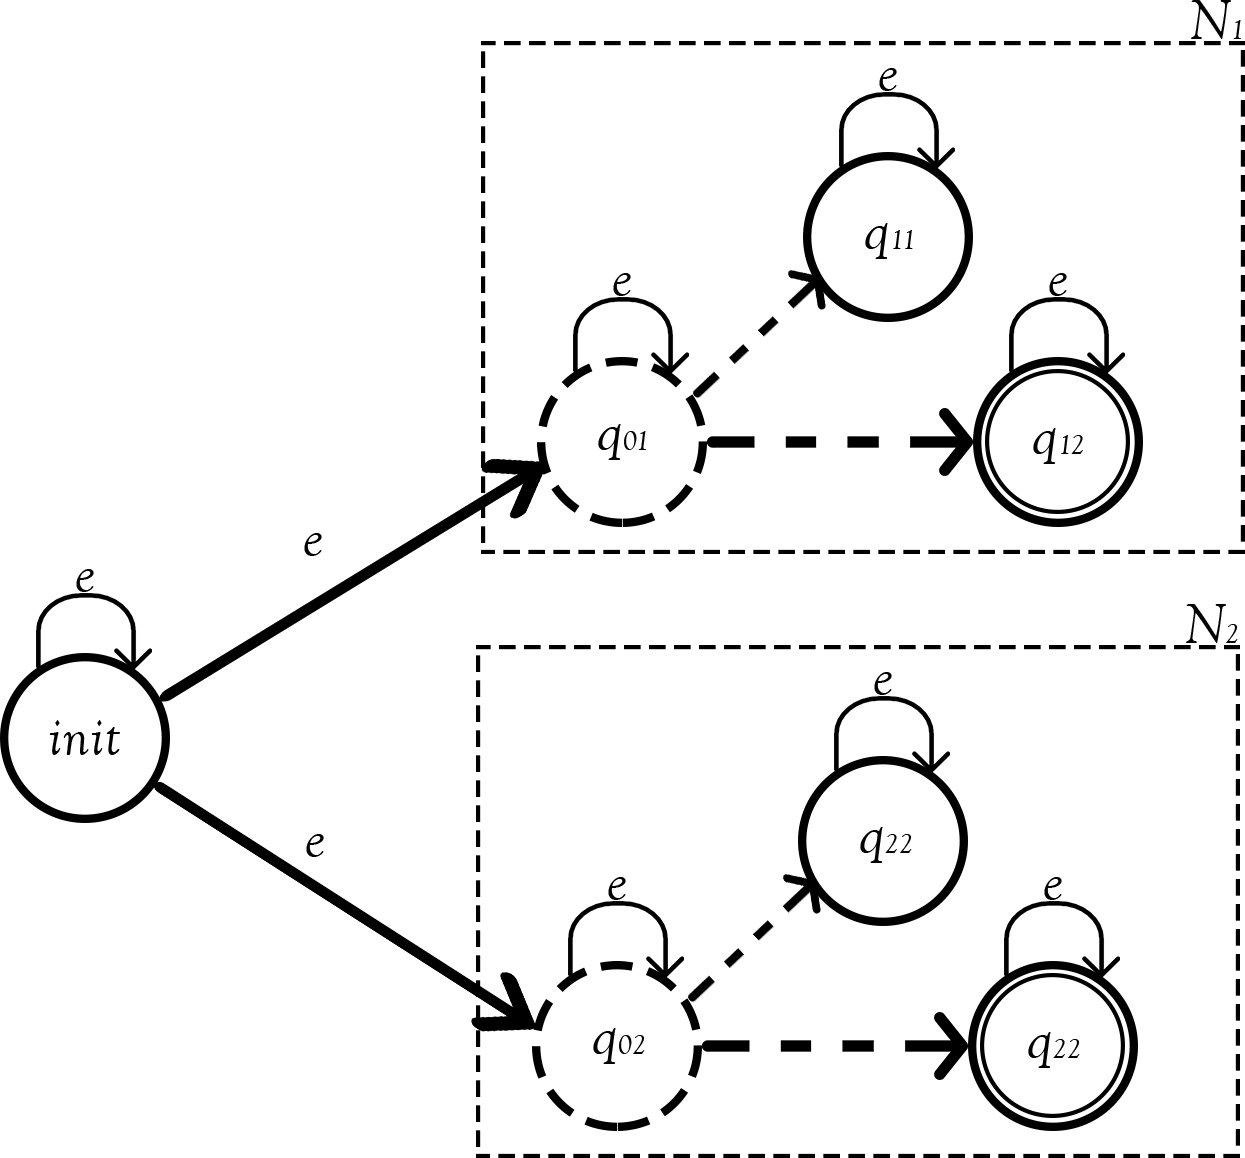
\includegraphics{union}\end{center}
      \item for \(e_1\cdot e_2\), we have \(M = (Q_1 \cup \{mid\}
        \cup Q_2,\ \Sigma^e,\ \delta,\ init,\ F_2)\) and graphically \begin{center}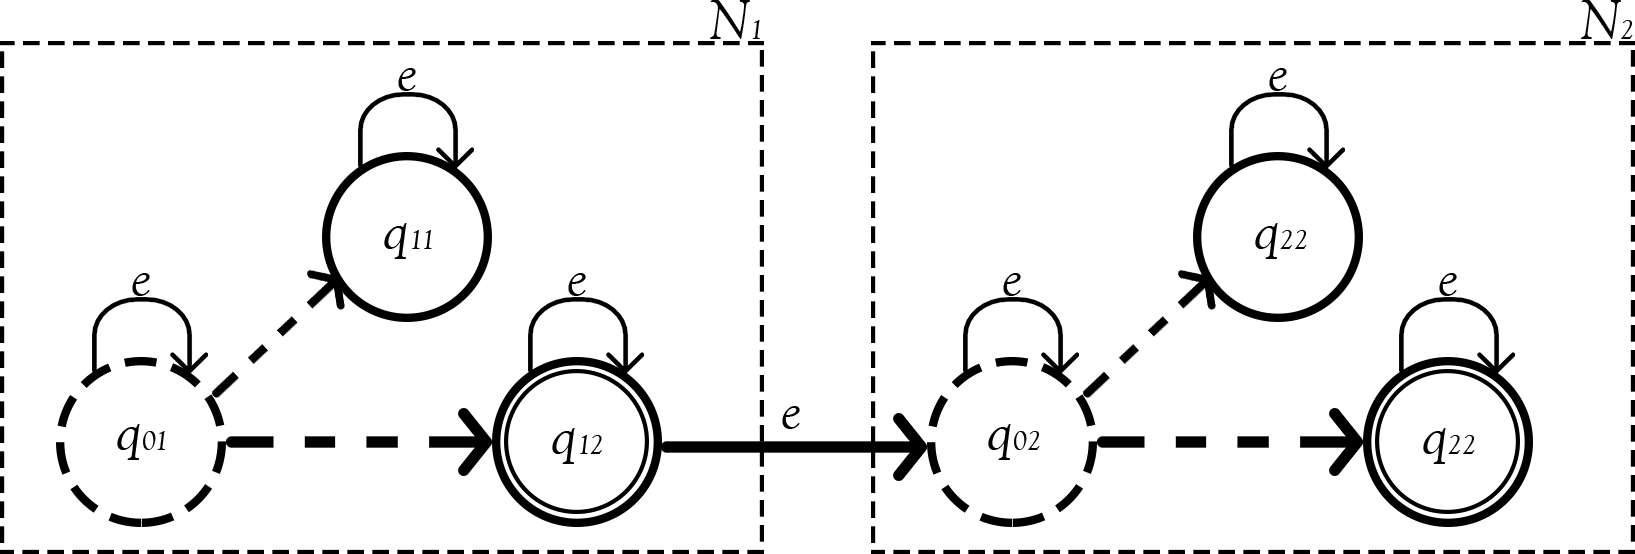
\includegraphics{concat}\end{center}
      \item for \(e_1^{\ *}\), we have \(M = (\{init\} \cup Q_1,\
        \Sigma^e,\ \delta,\ init,\ \{init\} \cup F_1)\) and
        graphically \begin{center}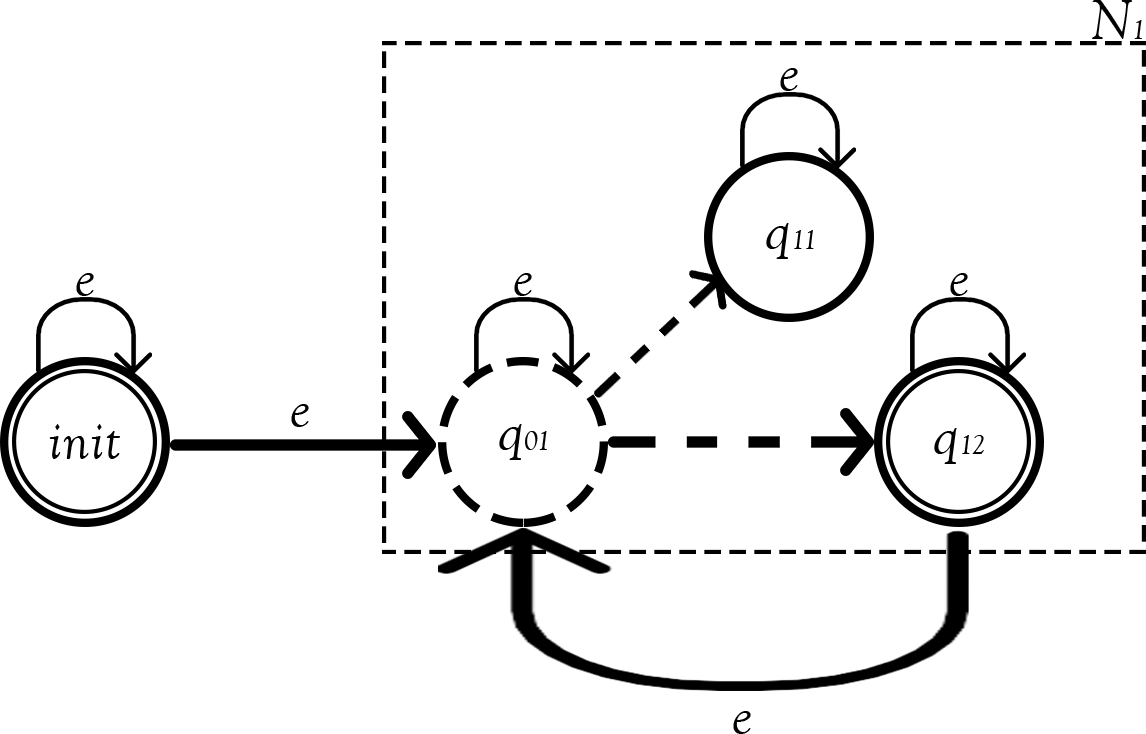
\includegraphics{star}\end{center}
     \end{enumerate}
\end{enumerate}
\end{defn}

\par Now, let us prove the correctness of the above translation by
proving their accepting languages are equal. The correctness proofs
can be found in \textbf{Correctness/RegExp-eNFA.agda}. 

\begin{thm} 
\noindent For any given regular expression, \(e\), its accepting
language is equal to the language accepted by an \(\epsilon\)-NFA
translated from \(e\) using Thompson's Construction, i.e. \(L(e) =
L(\)translated \(\epsilon\)-NFA\()\). 
\end{thm} 

\begin{proof}
\noindent We can prove the theorem by induction on regular
expressions. 

\par \noindent \textbf{Base cases.}\quad By \autoref{defn:thompson}, it is
obvious that the statement holds for \(\O\), \(\epsilon\) and
\(a\). 

\par \noindent \textbf{Induction hypothesis 1.}\quad For any two regular expressions
\(e_1\) and \(e_2\), let \(N_1 =
(Q_1,\ \delta_1,\ q_{01},\ F_1)\) and \(N_2 = (Q_2,\ \delta_2,\
q_{02},\ F_2)\) be their translated \(\epsilon\)-NFA 
respectively. We assume that \(L(e_1) = L(N_1)\) and \(L(e_2) =
L(N_2)\). 

\par \noindent \textbf{Inductive steps.}\quad There are three cases: 1)
\(e_1\ |\ e_2\), 2) \(e_1 \cdot e_2\) and 3) \(e_1^{\ *}\). 

\par \noindent 1) \textit{Case \((e_1\ |\ e_2)\)}: Let \(M = (Q,\ \delta,\ q_0,\ F) = (\{init\} \cup Q_1 \cup Q_2,\
\delta,\ init,\ F_1 \cup F_2)\) be its translated \(\epsilon\)-NFA. Then for any string \(w\), 

\par 1.1) if \((e_1\ |\ e_2)\) accepts \(w\), then by
\autoref{defn:regex} and \autoref{defn:lang_union},
either i) \(e_1\) accepts \(w\) or ii) \(e_2\) accepts \(w\). Assuming case i), then by
induction hypothesis, \(N_1\) also accepts \(w\) which implies that
there must exist an \(\epsilon\)-string of \(w\), \(w^e\), which can take \(q_{01}\)
to an accepting state \(q\) in \(N_1\). Now, consider another
\(\epsilon\)-string of \(w\), \(\epsilon w^e\), it can
take \(init\) to \(q\) in \(M\) because \(\epsilon\) can take \(init\)
to \(q_{01}\). Recall that \(q\) is an accepting
state in \(N_1\); therefore, \(q\) is also an accepting state in
\(M\). Now, we have proved that there exists an \(\epsilon\)-string
\(w\), \(\epsilon w^e\), that can take \(init\) to an accepting state
\(q\) in \(M\); and thus \(M\) accepts \(w\). The same argument also applies
to the case when \(e_2\) accepts \(w\). Since we have proved that
\(w \in L(e_1\ |\ e_2)\) implies \(w \in L(M)\) for any string \(w\);
therefore \(L(e_1\ |\ e_2) \subseteq L(M)\) is true; 

\par 1.2) if \(M\) accepts \(w\), then by \autoref{defn:enfa}, there must exist an
\(\epsilon\)-string of \(w\), \(w^e\), which can take \(init\) to an
accepting state \(q\) in \(M\). \(q\) must be different from \(init\) because
\(q\) is an accepting state but \(init\) is not. Now, by
\autoref{defn:thompson}, there are only two possible ways for \(init\) to reach \(q\) in \(M\), i)
via \(q_{01}\) or ii) via \(q_{02}\). Assuming case i), then the head of \(w^e\)
must be an \(\epsilon\) because it is the only alphabet that can take
\(init\) to \(q_{01}\). Furthermore, \(q\) is an
accepting state in \(M\); therefore, \(q\) is also an accepting
state in \(N_1\). Now, let \(w^e = \epsilon u^e\), we have proved that
there exists an \(\epsilon\)-string \(w\), \(u^e\), which can take
\(q_{01}\) to an accepting state \(q\) in \(N_1\); and thus \(N_1\)
accepts \(w\). By induction hypothesis, \(e_1\) also accepts \(w\);
therefore, we have \(w \in L(e_1\ |\ e_2)\). The same argument also
applies to case ii). Since we have proved that \(w \in L(M)\) implies
\(w \in L(e_1\ |\ e_2)\) for any string \(w\); therefore \(L(e_1\ |\
e_2) \supseteq L(M)\) is true; 

\par 1.3) combining 1.1 and 1.2, we have \(L(e_1\ |\ e_2) = L(M)\). 

\par \noindent 2) \textit{Case \((e_1 \cdot e_2)\)}: Let \(M = (Q,\
\delta,\ q_0,\ F) = (Q_1 \cup \{mid\} \cup Q_2,\ \delta,\ q_{01},\
F_2)\) be its translated \(\epsilon\)-NFA. Then for any string
\(w\), 

\par 2.1) if \((e_1 \cdot e_2)\) accepts \(w\), then by
\autoref{defn:regex} and \autoref{defn:lang_con}, there must exist a string \(u \in L(e_1)\) and a string \(v \in L(e_2)\) such that \(w
= uv\). By induction hypothesis, \(N_1\) accepts \(u\) and \(N_2\)
accepts \(v\). Therefore, there must exist i) an \(\epsilon\)-string
of \(u\), \(u^e\), which can take \(q_{01}\) to an accepting state \(q_1\) in
\(N_1\) and ii) an \(\epsilon\)-string of \(v\), \(v^e\), which can take
\(q_{02}\) to an accepting state \(q_2\) in \(N_2\). Now, let us
consider another \(\epsilon\)-string of \(w\), \(u^e\epsilon \epsilon
v^e\), it can take \(q_{01}\) to \(q_2\) in \(M\) because \(u^e\) takes
\(q_{01}\) to \(q_1\), \(\epsilon\) takes \(q_1\) to \(mid\), another
\(\epsilon\) takes \(mid\) to \(q_{02}\) and \(v^e\) takes \(q_{02}\)
to \(q_2\). Furthermore, \(q_2\)
is also an accepting state in \(M\) because \(q_2\) is an accepting
state in \(N_2\). Therefore, we have proved that \(M\) accepts \(w\). 
Since we have proved that \(w \in L(e_1 \cdot e_2)\) implies 
\(w \in L(M)\) for any string \(w\); therefore \(L(e_1 \cdot e_2) \subseteq L(M)\) is true; 

\par 2.2) if \(M\) accepts \(w\), then by \autoref{defn:enfa}, there must
exist an \(\epsilon\)-string of \(w\), \(w^e\), which can take
\(q_{01}\) to an accepting state \(q\) in \(M\). Since \(q\) is an
accepting state in \(M\); therefore, \(q\) must be in \(Q_2\). The only possible way for
\(q_{01}\) to reach \(q\) is by going through the state \(mid\). This
implies that there must exist i) an \(\epsilon\)-string of \(u^e\), which can take
\(q_{01}\) to an accepting state \(q_1\) in \(N_1\) and ii) an
\(\epsilon\)-string \(v^e\) which can take \(q_{02}\) to \(q_2\) in
\(N_1\) and \(w^e = u^ev^e\). Let \(u\) and \(v\) be the normal strings of \(u^e\) and
\(v^e\) respectively, then we have \(u \in L(N_1)\), \(v \in L(N_2)\) and \(w = uv\). Now, by induction
hypothesis, \(e_1\) accepts \(u\) and \(e_2\) accepts \(v\); and thus
\(e_1 \cdot e_2\) accepts \(w\). Since we have proved that \(w \in
L(M)\) implies \(w \in L(e_1 \cdot e_2)\) for any string \(w\); therefore \(L(e_1 \cdot
e_2) \supseteq L(M)\) is true; 

\par 2.3) combining 2.1 and 2.2, we have \(L(e_1 \cdot e_2) = L(M)\). 

\par \noindent 3) \textit{Case \(e_1^{\ *}\)}: Let \(M = (Q,\ \delta,\ q_0,\
F) = (Q_1 \cup \{mid\} \cup Q_2,\ \delta,\ q_{01},\ F_2)\) be its
translated \(\epsilon\)-NFA. Then for any string \(w\), 

\par 3.1) if \((e_1^{\ *})\) accepts \(w\), then by \autoref{defn:regex}
and \autoref{defn:lang_star}, there must exist a number \(n\) such
that \(w \in L(e_1)^n\). Now, let us do induction on \(n\). 

\par \quad \textbf{Base case.} \quad When \(n = 0\), then language
\(L^0\) can only accept the empty string \(\epsilon\); and thus \(w =
\epsilon\). From \autoref{defn:thompson}, it is obvious that \(M\)
accepts \(\epsilon\). 

\par \quad \textbf{Induction hypothesis 2.} \quad Suppose there exists a number \(k\) such that \(w
\in L(e_1)^k\), then \(w\) is also accepted by \(M\). 

\par \quad \textbf{Induction steps.} \quad When \(n = k + 1\), by
\autoref{defn:lang_con} and \autoref{defn:lang_power}, there must
exist a string \(u \in L(e_1)\) and a string \(v \in L(e_1)^k\) such
that \(w=uv\). By induction hypothesis (1), we have \(u
\in L(N_1)\) which implies that there must exist an \(\epsilon\)-string
\(u\), \(u^e\), that can take \(q_{01}\) to an accepting state \(q\)
in \(N_1\). Since \(q\) is an accepting state; an \(\epsilon\)
alphabet can take \(q\) back to \(q_{01}\). Furthermore, by induction
hypothesis (2), \(M\) also accepts \(v\) which implies that there
exists an \(\epsilon\)-string of \(v\), \(v^e\), that can take
\(init\) to an accepting state \(p\). Since the only
alphabet that can take \(init\) to \(q_{01}\) is \(\epsilon\); therefore,
\(v^e\) must be in the form of \(\epsilon v'^e\). Now, we have proved
that there exists an \(\epsilon\) string of \(w\), \(\epsilon u^e\epsilon v'^e\), that can
take \(init\) to an accepting state \(p\) in \(M\); and thus \(M\)
accepts \(w\). Since we have proved that \(w \in L(e_1^{\ *})\) implies
\(w \in L(M)\) for any string \(w\); therefore \(L(e_1^{\ *}) \subseteq L(M)\) is true; 

\par 3.2) if \(M\) accepts \(w\), then by \autoref{defn:enfa}, there must exist an
\(\epsilon\)-string \(w\), \(w^e\), that can take \(init\) to an accepting
state \(q\) using \(n\) transitions in \(M\).  If \(init = q\), then \(w\) must be an empty
string. By \autoref{defn:thompson}, it is obvious that
the empty string is accepted by \(e_1^{\ *}\). If \(init \neq q\),
then there are only two possible ways for \(init\)
to reach \(q\): 1) from \(init\) to \(q\) without any
transition that takes an accepting state in \(M\) back
to \(q_{01}\), we say that this path has no loops and 2) from \(init\)
to \(q\) with at least one transition that takes an accepting state in \(M\) back
to \(q_{01}\), we say that this path has loop. 
\par \quad \textit{Case 1}: Since \(q \neq init\), then \(w^e\) must
be in the form of \(\epsilon w'^e\). Recall that the path has no loops, it is
obvious that \(N_1\) accepts \(w\). Therefore by
induction hypothesis (1), \(e_1\) accepts \(w\) and thus \(e_1^{\ *}\)
also accepts \(w\). 
\par \quad \textit{Case 2}: Since \(q \neq init\), then \(w^e\) must
be in the form of \(\epsilon w'^e\). Recall that the path has loops, we
can separate \(w'^e\) into two parts: 1) an \(\epsilon\)-string
\(u^e\) that takes \(init\) to an accepting state \(p\) without loops
and 2) an \(\epsilon\)-string \(v^e\) that takes \(p\) to
\(q_{01}\) to \(q\) with loops. Let \(u\) and \(v\) be the normal
string of \(u^e\) and \(v^e\) respectively, then it is obvious that
\(w = uv\). By \textit{case 1}, \(e_1\) accepts \(u\). Now, consider
the path from \(q_{01}\) to \(q\). The path must have less than \(n\)
transitions; therefore, we can prove by induction the there must exist a number \(k\) such that
\(L(e_1)^k\) accepts \(v\). Combining the above proofs, we have \(w \in
L(e_1^{\ *})\). 
\par \quad Since we have proved that \(w \in L(M)\) implies \(w \in L(e_1^{\
  *})\) for any string \(w\); therefore \(w \in L(e_1^{\ *}) \supseteq L(M)\) is true; 

\par 3.3) combining 3.1 and 3.2, we have \(L(e_1^{\ *}) = L(M)\). 

\par \noindent Therefore, by induction, \(L(e) = L(\)translated
\(\epsilon\)-NFA\()\) is true for all any regular expression \(e\). 
\end{proof}


\subsection{Non-deterministic Finite Automata}
\par Although the definition of NFA is very similar to that of
\(\epsilon\)-NFA, we will still give the definition of NFA
separately. The type of NFA is defined in \textbf{NFA.agda} along with
its operations and properties. 

\begin{defn}
\noindent A NFA is a 5-tuple \(M = (Q
,\ \Sigma,\ \delta,\ q_0,\ F)\), where
\begin{enumerate}[nolistsep]
  \item \(Q\) is a finite set of states;
  \item \(\Sigma\) is the set of alphabets;
  \item \(\delta\) is a mapping from \(Q \times \Sigma\) to
    \(\mathcal P \left({Q}\right)\) that defines the behaviour of the automata;
  \item \(q_0\) in \(Q\) is the initial state;
  \item \(F \subseteq Q\) is the set of accepting states. 
\end{enumerate}
\end{defn}

\par It is formalised as a record in Agda as shown below: 

\begin{lstlisting}[mathescape=true,xleftmargin=.3\textwidth]
record NFA : Set$_1$ where
  field
    Q      : Set
    $\delta$       : Q $\to$ $\Sigma$ $\to$ DecSubset Q
    q$_0$      : Q
    F      : DecSubset Q
    Q?     : DecEq Q
    |Q|-1  : $\mathbb{N}$
    It     : Vec Q (suc |Q|-1)
    $\forall$q$\in$It    : (q : Q) $\to$ (q $\in^V$ It)
    unique : Unique It
\end{lstlisting}

\par The set of alphabets \(\Sigma\) is passed into the module as a
parameter. Together with \(Q\), \(\delta\),
\(q_0\) and \(F\), these five fields correspond to the 5-tuple
NFA. The other extra fields are used in powerset construction. They
are \(Q?\) -- the decidable equality of \(Q\);
\(|Q|-1\) -- the number of states minus 1; \(It\) -- a vector containing every state in \(Q\); \(\forall q\in It\)
-- a proof that every state in \(Q\) is also in the vector
\(It\); and \(unique\) -- a proof that there is no repeating elements in
\(It\). 

\par Now, before we can define the accepting language of a given
NFA, we need to define several operations of NFA. 

\begin{defn}
\noindent A configuration is composed of a state and an alphabet from
\(\Sigma\), i.e. \(C = Q \times \Sigma\). 
\end{defn}

\begin{defn}
\noindent A move in an NFA \(N\) is
represented by a binary function (\(\vdash\)) on two configurations. We say
that for all \(w \in \Sigma^*\) and \(a \in \Sigma\), \((q, aw)
\vdash (q' , w)\) if and only if \(q' \in \delta (q , a)\). 
\end{defn}

\par The binary function is defined in Agda as follow: 
\begin{lstlisting}[mathescape=true,xleftmargin=.3\textwidth]
  _$\vdash$_ : (Q $\times$ $\Sigma$ $\times$ $\Sigma^*$) $\to$ (Q $\times$ $\Sigma^*$) $\to$ Set
  (q , a , w) $\vdash$ (q' , w') = w $\equiv$ w' $\times$ q' $\in^d$ $\delta$ q a
\end{lstlisting}

\begin{defn}
\noindent Suppose \(C\) and \(C'\) are configurations. We say that \(C \vdash^0 C'\) if and only
if \(C = C'\); and \(C_0 \vdash^k C_k\) for any \(k \geq 1\) if and only if there exists a chain of
configurations \(C_1, C_2, ..., C_{k-1}\) such that \(C_i \vdash C_{i+1}\) for all \(0 \leq i < k\). 
\end{defn}

\par It is defined as a recursive function in Agda as follow: 
\begin{lstlisting}[mathescape=true,xleftmargin=.3\textwidth]
  _$\vdash^k$_-_ : (Q $\times$ $\Sigma^*$) $\to$ $\mathbb{N}$ $\to$ (Q $\times$ $\Sigma^*$) $\to$ Set
  (q , w) $\vdash^k$ zero  - (q' , w')
    = q $\equiv$ q' $\times$ w $\equiv$ w'
  (q , w) $\vdash^k$ suc n - (q' , w') 
    = $\exists$[ p $\in$ Q ] $\exists$[ a $\in$ $\Sigma$ ] $\exists$[ u $\in$ $\Sigma^*$ ]
      (w $\equiv$ a :: u $\times$ (q , a , u) $\vdash$ (p , u) $\times$ (p , u) $\vdash^k$ n - (q' , w'))
\end{lstlisting}

\begin{defn}
\noindent We say that \(C \vdash^* C'\) if and only
if there exists a number of chains \(n\) such that \(C \vdash^n C'\). 
\end{defn}

\par Its corresponding type is defined as follow: 
\begin{lstlisting}[mathescape=true,xleftmargin=.3\textwidth]
  _$\vdash^*$_ : (Q $\times$ $\Sigma^*$) $\to$ (Q $\times$ $\Sigma^*$) $\to$ Set
  (q , w) $\vdash^*$ (q' , w') = $\exists$[ n $\in$ $\mathbb{N}$ ] (q,w) $\vdash^k$ n - (q',w')
\end{lstlisting}

\begin{defn}
\noindent For any string \(w\), it is accepted by an NFA
if and only \(w\) can take \(q_0\) to an accepting state \(q\). Therefore, the
accepting language of an NFA is given by the set \(\{\ w\ |\ \exists q\in F.\ (q_0,w) \vdash^* (q,\epsilon)\ \}\). 
\end{defn}

\par The corresponding formalisation in Agda is as follow: 
\begin{lstlisting}[mathescape=true,xleftmargin=.3\textwidth]
  L$^N$ : NFA $\to$ Language
  L$^N$ nfa = $\lambda$ w $\to$ 
            $\exists$[ q $\in$ Q ] (q $\in^d$ F $\times$ (q$_0$ , w) $\vdash^*$ (q , [])))
\end{lstlisting} 

\par Now we can formulate the translation of \(\epsilon\)-NFA to NFA
by removing all the \(\epsilon\)-transitions. 


\subsection{Removing \(\epsilon\)-transitions}
\par The translation of \(\epsilon\)-NFA to NFA is defined in
\textbf{Translation/eNFA-NFA.agda}. In order to remove all the \(\epsilon\)-transitions, we need to
know whether a state \(q\) can reach another state \(q'\) by only
\(\epsilon\)-transitions. Let us begin by defining such a predicate. 

\begin{defn}
\noindent Let us first define a binary relation on states. We say that
\(q \to_\epsilon^0 q'\) if and only if
\(q\) is equal to \(q'\); and \(q \to_\epsilon^k q'\) for \(k \geq
1\) if and only if there exists a state \(p\) such that \(p \in
\delta (q,\epsilon)\) and \(p \to_\epsilon^{k-1} q'\). We call this
an \(\epsilon\)-path from \(q\) to \(q'\).
\end{defn}

\par It is defined as a recursive function in Agda as follow:
\begin{lstlisting}[mathescape=true,xleftmargin=.3\textwidth]
_$\to_\epsilon^k$_-_ : Q $\to$ $\mathbb{N}$ $\to$ Q $\to$ Set
q $\to_\epsilon^k$ zero - q' = q $\equiv$ q'
q $\to_\epsilon^k$ suc n - q' = $\exists$[ p $\in$ Q ] ( p $\in^d$ $\delta$ q E $\times$ p $\to_\epsilon^k$ n - q' )
\end{lstlisting}

\begin{defn}
\noindent We say that \(q \to_\epsilon^* q'\) if and only if there
exists an \(\epsilon\)-path from \(q\) to \(q'\) with \(n\) transitions, i.e. \(\exists n.\ q \to_\epsilon^n q'\). 
\end{defn}

\par The corresponding type is as follow: 
\begin{lstlisting}[mathescape=true,xleftmargin=.3\textwidth]
_$\to_\epsilon^*$_ : Q $\to$ Q $\to$ Set
q $\to_\epsilon^*$ q' = $\exists$[ n $\in$ $\mathbb{N}$ ] q $\to_\epsilon^k$ n - q'
\end{lstlisting}

\par Now we have to prove that for any two states \(q\) and \(q'\), 
\(q \to_\epsilon^* q'\) is decidable. However, it is not possible to
prove it directly because the set of natural numbers is
infinite. Therefore, we will introduce an algorithm that computes the
\(\epsilon\)-closure for a state and prove that for any two states
\(q\) and \(q'\), \(q \to_\epsilon^* q'\) if and only if \(q'\) is in
the \(\epsilon\)-closure of \(q\). By proving they are equivalent, we
will have proved the decidability of \(q \to_\epsilon^* q'\). 

\begin{defn}
\noindent For any given state \(q\), the \(\epsilon\)-closure of
\(q\), i.e. \(\epsilon\hyphen -closure(q)\) is obtained by: 
\begin{enumerate}[nolistsep]
  \item put \(q\) into a subset \(S\), i.e. \(S = \{q\}\)
  \item loop for \(|Q| - 1\) times: 
  \begin{enumerate}
    \item for every state \(p\) in \(S\), if \(\epsilon\) can take
      \(p\) to another state \(r\), i.e. \(r \in
        \delta (p,\epsilon)\), then put \(r\) into \(S\). 
  \end{enumerate}
  \item the result subset \(S\) is the \(\epsilon\)-closure of \(q\)
\end{enumerate}
\end{defn}

\begin{lem}
\noindent For any two states \(q\) and \(q'\), \(q \to_\epsilon^* q'\)
if and only if \(q' \in \epsilon\hyphen -closure(q)\). 
\end{lem}

\begin{proof}
\noindent To prove the lemma, we have to prove that \(q \to_\epsilon^*
q'\) implies \(q' \in \epsilon\hyphen closure(q)\) and \(q' \in
\epsilon\hyphen closure(q)\) implies \(q \to_\epsilon^* q'\). 

\par 1) If \(q \to_\epsilon^* q'\), then there must exist a
number \(n\) such that \(\epsilon^n\) can take \(q\) to \(q'\). If
\(n < |Q|\), then it is obvious that \(q' \in
\epsilon\hyphen closure(q)\) is true. If \(n \geq |Q|\), the
\(\epsilon\)-path from \(q\) to \(q'\) must have loop(s) inside. By
removing the loop(s), the equivalent \(\epsilon\)-path must have at
most \(|Q|-1\) \(\epsilon\)-transitions. Therefore, \(q' \in
\epsilon\hyphen closure(q)\) is true. 

\par 2) If \(q' \in \epsilon\hyphen closure(q)\), it is obvious
that \(q \to_\epsilon^{|Q|-1} q'\) must be true. 
\end{proof}

\par Since we have proved that they are equivalent, therefore the
decidability of \(q \to_\epsilon^* q'\) follows. Now, let us define
the translation of \(\epsilon\)-NFA to NFA using \(q \to_\epsilon^* q'\). 
 
\begin{defn}
\label{defn:remove_epsilon}
\noindent For a given \(\epsilon\)-NFA, \((Q,\ \delta,\
q_0,\ F)\), its translated NFA will be \((Q,\ \delta',\ q_0,
F')\) where
\begin{itemize}[nolistsep]
  \item \(\delta'(q,a) = \delta (q,a) \cup \{q'\ |\ \exists p\in Q.\
      q \to_\epsilon^* p \wedge q' \in \delta (p,a)\}\); and
  \item \(F' = F \cup \{q\ |\ \exists p\in Q.\ q \to_\epsilon^* p \wedge p
      \in F\} \). 
\end{itemize}
\end{defn}

\par Now, let us prove the correctness of the above translation by proving their accepting languages
are equal. The correctness proofs can be found in Correctness/eNFA-NFA.agda.

\begin{thm}
\noindent For any \(\epsilon\)-NFA, its accepting language is equal to
the accepted language of its translated NFA, i.e. \(L(\epsilon\)-NFA\()
= L(\)translated NFA\()\). 
\end{thm}

\begin{proof}
\noindent For a given \(\epsilon\)-NFA, \(\epsilon N = (Q,\ \delta,\ q_0,\
F)\), let its translated NFA be \(N = (Q,\ \delta',\ q_0,\ F')\)
according to \autoref{defn:remove_epsilon}. To
prove the theorem, we have to prove \(L(\epsilon N) \subseteq
L(N)\) and \(L(\epsilon N) \supseteq L(N)\). For any string \(w\), 

\par \noindent 1) if \(\epsilon N\) accepts \(w\), then there must exist an
\(\epsilon\)-string of \(w\), \(w^e\), that can take \(q_0\) to an
accepting state \(q\) in \(n\) transitions. There are three
possibilities: a) the last transition in the path is not an
\(\epsilon\)-transition, b) the path is divided into three parts, the
first part from \(q_0\) to a state \(p\) with less than \(n\)
transitions; the second part from \(p\) to a state \(p_1\) with an
alphabet \(a\) and the third part from \(p_1\) to \(q\) with only
\(\epsilon\)-transitions and c) the path from \(q_0\)
to \(q\) consists of only \(\epsilon\)-transitions.

\par \textit{Case a}: There must exist a state \(p\) and an
\(\epsilon\)-string, \(u^e\), and an alphabet \(a\) such that \(u^e\)
can take \(q_0\) to \(p\) in less than \(n\) transitions, the alphabet
\(a\) can take \(p\) to \(q\) and \(w^e = u^ea\). We can prove by
induction that the normal string of \(u^e\), \(u\), can take
\(q_0\) to \(p\) in \(N\) and \(w = ua\). Therefore, we have proved that \(w\) can
take \(q_0\) to \(q\) in \(N\) and thus \(N\) accepts \(w\). 

\par \textit{Case b}: There must exist two states \(p\) and \(p_1\), an
\(\epsilon\)-string of \(w\), \(u^e\), and an alphabet \(a\) such
that \(u^e\) can take \(q_0\) to \(p\) in less than \(n\) transitions,
\(a\) can take \(p\) to \(p_1\), \(p_1 \to_\epsilon^* q\) and \(w = ua\). We can prove by
induction that the normal string of \(u^e\), \(u\), can take \(q_0\) to \(p\) in
\(N\). Furthermore, \(p_1\) must be an accepting state in \(N\)
because it can be transited to an accepting state \(q\) with only
\(\epsilon\)-transitions. Therefore, we have proved that \(w\) can take \(q_0\) to an
accepting state \(p_1\) in \(N\) and thus \(N\) accepts \(w\). 

\par \textit{Case c}: If the path from \(q_0\)
to \(q\) consists of only \(\epsilon\)-transitions, then \(q_0
\to_\epsilon^* q\); therefore, \(q_0\) is also an accepting
state. The accepted string must consist of \(\epsilon\) only;
therefore, \(w = \epsilon\). It is obvious that \(N\) accepts
\(\epsilon\). 

\par \noindent 2) if \(N\) accepts \(w\), then \(w\) can take \(q_0\) to an
accepting state \(q\). Since \(q\) is an accepting state, then \(q\)
is also an accepting state in \(\epsilon N\) or there exist a state
\(p\) such that \(q \to_\epsilon^* p\) and \(p \in F\). For the former
case, since \(w\) is also an \(\epsilon\)-string of itself; therefore,
it is obvious that \(\epsilon N\) also accepts \(w\). For the latter
case, suppose the path from \(q\) to \(p\) has \(n\)
\(\epsilon\)-transitions, then we can append \(n\) \(\epsilon's\) to
\(w\) such that \(w\epsilon^n\) can take \(q_0\) to \(p\) in
\(\epsilon N\). Therefore \(\epsilon N\) accepts \(w\). 
\end{proof}

\subsection{Deterministic Finite Automata}
\par The type of DFA is defined in \textbf{DFA.agda} along with its
operations and properties. 

\begin{defn}
\noindent A DFA is a 5-tuple \(M = (Q
,\ \Sigma,\ \delta,\ q_0,\ F)\), where
\begin{enumerate}[nolistsep]
  \item \(Q\) is a finite set of states;
  \item \(\Sigma\) is the set of alphabets;
  \item \(\delta\) is a mapping from \(Q \times \Sigma\) to \(Q\) that defines the behaviour of the automata;
  \item \(q_0\) in \(Q\) is the initial state;
  \item \(F \subseteq Q\) is the set of accepting states. 
\end{enumerate}
\end{defn}

\par It is formalised as a record in Agda as shown below: 

\begin{lstlisting}[mathescape=true,xleftmargin=.3\textwidth]
record NFA : Set$_1$ where
  field
    Q      : Set
    $\delta$       : Q $\to$ $\Sigma$ $\to$ DecSubset Q
    q$_0$      : Q
    F      : DecSubset Q
    _$\approx$_ : Q $\to$ Q $\to$ Set
    $\approx\hyphen$isEquiv : IsEquivalence _$\approx$_
    $\delta\hyphen$lem   : $\forall$ {q} {p} a $\to$ q $\approx$ p $\to$ $\delta$ q a $\approx$ $\delta$ p a
    F$\hyphen$lem   : $\forall$ {q} {p}   $\to$ q $\approx$ p $\to$ q $\in^d$ F $\to$ p $\in^d$ F
\end{lstlisting}

\par The set of alphabets \(\Sigma\) is passed into the module as a
parameter. Together with \(Q\), \(\delta\),
\(q_0\) and \(F\), these five fields correspond to the 5-tuple
DFA. The other extra fields are used in proving its decidability. They
are \(\_\approx\_\) -- an equivalence relation on states;
\(\approx\hyphen isEquiv\) -- a proof that the relation \(\approx\) is
an equivalence relation; \(\delta\hyphen lem\) -- a proof that for any
alphabet \(a\) and any two states \(q\) and \(p\), if \(q \approx p\)
then \(\delta (q,a) \approx \delta (p,a)\); and \(F\hyphen lem\) -- a
proof that for any two states \(q\) and \(p\), if \(q \approx p\) and
\(q\) is an accepting state, then \(p\) is also an accepting state. 

\par Now, before we can define the accepting language of a given
DFA, we need to define several operations of DFA. 

\begin{defn}
\noindent A configuration is composed of a state and an alphabet from
\(\Sigma\), i.e. \(C = Q \times \Sigma\). 
\end{defn}

\begin{defn}
\noindent A move in an NFA \(N\) is
represented by a binary function (\(\vdash\)) on two configurations. We say
that for all \(w \in \Sigma^*\) and \(a \in \Sigma\), \((q, aw)
\vdash (q' , w)\) if and only if \(q' = \delta (q , a)\). 
\end{defn}

\par The binary function is defined in Agda as follow: 
\begin{lstlisting}[mathescape=true,xleftmargin=.3\textwidth]
  _$\vdash$_ : (Q $\times$ $\Sigma$ $\times$ $\Sigma^*$) $\to$ (Q $\times$ $\Sigma^*$) $\to$ Set
  (q , a , w) $\vdash$ (q' , w') = w $\equiv$ w' $\times$ q' $\approx$ $\delta$ q a
\end{lstlisting}

\begin{defn}
\noindent Suppose \(C\) and \(C'\) are configurations. We say that \(C \vdash^0 C'\) if and only
if \(C = C'\); and \(C_0 \vdash^k C_k\) for any \(k \geq 1\) if and only if there exists a chain of
configurations \(C_1, C_2, ..., C_{k-1}\) such that \(C_i \vdash C_{i+1}\) for all \(0 \leq i < k\). 
\end{defn}

\par It is defined as a recursive function in Agda as follow: 
\begin{lstlisting}[mathescape=true,xleftmargin=.3\textwidth]
  _$\vdash^k$_-_ : (Q $\times$ $\Sigma^*$) $\to$ $\mathbb{N}$ $\to$ (Q $\times$ $\Sigma^*$) $\to$ Set
  (q , w) $\vdash^k$ zero  - (q' , w')
    = q $\equiv$ q' $\times$ w $\equiv$ w'
  (q , w) $\vdash^k$ suc n - (q' , w') 
    = $\exists$[ p $\in$ Q ] $\exists$[ a $\in$ $\Sigma$ ] $\exists$[ u $\in$ $\Sigma^*$ ]
      (w $\equiv$ a :: u $\times$ (q , a , u) $\vdash$ (p , u) $\times$ (p , u) $\vdash^k$ n - (q' , w'))
\end{lstlisting}

\begin{defn}
\noindent We say that \(C \vdash^* C'\) if and only
if there exists a number of chains \(n\) such that \(C \vdash^n C'\). 
\end{defn}

\par Its corresponding type is defined as follow: 
\begin{lstlisting}[mathescape=true,xleftmargin=.3\textwidth]
  _$\vdash^*$_ : (Q $\times$ $\Sigma^*$) $\to$ (Q $\times$ $\Sigma^*$) $\to$ Set
  (q , w) $\vdash^*$ (q' , w') = $\exists$[ n $\in$ $\mathbb{N}$ ] (q,w) $\vdash^k$ n - (q',w')
\end{lstlisting}

\begin{defn}
\noindent For any string \(w\), it is accepted by an DFA
if and only \(w\) can take \(q_0\) to an accepting state \(q\). Therefore, the
accepting language of an DFA is given by the set \(\{\ w\ |\ \exists q\in F.\ (q_0,w) \vdash^* (q,\epsilon)\ \}\). 
\end{defn}

\par The corresponding formalisation in Agda is as follow: 
\begin{lstlisting}[mathescape=true,xleftmargin=.3\textwidth]
  L$^D$ : DFA $\to$ Language
  L$^D$ dfa = $\lambda$ w $\to$ 
            $\exists$[ q $\in$ Q ] (q $\in^d$ F $\times$ (q$_0$ , w) $\vdash^*$ (q , [])))
\end{lstlisting} 

\par Now we can formulate the translation of NFA to DFA
by powerset construction. 


\subsection{Powerset Construction}
\par The translation of NFA to DFA is defined in
\textbf{Translation/NFA-DFA.agda}. 

\begin{defn}
\label{defn:powerset}
\noindent For any given NFA, \((Q,\ \delta,\ q_0,\ F)\), its
translated DFA will be \((\mathcal P \left({Q}\right),\ \delta',\ \{q_0\},\ F')\) where
\begin{itemize}[nolistsep]
  \item \(\delta'(qs,a) = \{q'\ |\ \exists q\in Q.\ q \in qs \wedge q'
    \in \delta (q,a)\}\) and 
  \item \(F' = \{qs\ |\ \exists q\in Q.\ q \in qs \wedge q \in F\}\). 
\end{itemize}
\end{defn}

\par Now, before proving their accepting languages are equal, we first
need to prove the following lemmas. Note that the theorems and proofs below can be found in
\textbf{Correctness/NFA-DFA.agda}. 

\begin{lem}
\label{lem:nfa<dfa}
\noindent Let a NFA be \(N = (Q,\ \delta,\ q_0,\ F)\) and its
translated DFA be \(D = (\mathcal P \left({Q}\right),\ \delta',\ {q_0},
F')\) according to \autoref{defn:powerset}. For any string \(w\), if \(w\) can take \(q_0\) to a state
\(q\) with \(n\) transitions in \(N\), then there must exist a subset \(qs\) such that \(q
\in qs\) and \(w\) can take \(\{q_0\}\) to \(qs\) in \(D\). 
\end{lem}

\begin{proof}
\noindent We can prove the lemma by induction on \(n\).
\par \noindent \textbf{Base case.}\quad If \(n = 0\), then \(q_0 = q\)
and \(w = \epsilon\). It is obvious that the statement holds.

\par \noindent \textbf{Induction hypothesis.}\quad For any string \(w\), if \(w\) can take \(q_0\) to a state
\(q\) with \(k\) transitions in \(N\), then there exists a subset \(qs\) such that \(q
\in qs\) and \(w\) can take \(\{q_0\}\) to \(qs\) in \(D\). 

\par \noindent \textbf{Induction step.}\quad If \(n = k + 1\), then
\(w\) can take \(q_0\) to a state \(q\) by \(k + 1\) transitions. Let
\(w = w'a\) where \(a\) is an alphabet, then \(w'\) can take \(q_0\)
to a state \(p\) by \(k\) transitions and \(a\) can take \(p\) to
\(q\). By induction hypothesis, there must exist a subset \(ps\) such that \(p
\in ps\) and \(w'\) can take \(\{q_0\}\) to \(ps\) in \(D\). Furthermore, since \(a\) can take \(p\) to \(q\), then \(a\) must be
able to take \(ps\) to a subset \(qs\) where \(q \in qs\). Therefore,
there exists a subset \(qs\) such that \(q \in qs\) and \(w\) can take
\(\{q_0\}\) to \(qs\) and thus the statement is true. 
\end{proof}


\begin{lem}
\label{lem:nfa>dfa}
\noindent Let a NFA be \(N = (Q,\ \delta,\ q_0,\ F)\) and its
translated DFA be \(D = (\mathcal P \left({Q}\right),\ \delta',\ {q_0},
F')\) according to \autoref{defn:powerset}. For any string \(w\) and any
two states \(qs\) and \(ps\) in \(\mathcal P \left({Q}\right)\), if
\((qs,w) \vdash^n (ps,\epsilon)\) then \(ps =
\{p\ |\ \exists q\in qs.\ (q,w) \vdash^n (p,\epsilon)\}\). 
\end{lem}

\begin{proof}
\noindent We can prove the lemma by induction on \(n\). 

\par \noindent \textbf{Base case.}\quad If \(n = 0\), then \(qs = ps\)
and \(w = \epsilon\). Then for any state \(p\) in \(Q\), 
\par 1) if \(p \in ps\), then \(p\) also in \(qs\). It is obvious that
\((p,\epsilon) \vdash^0 (p, \epsilon)\) is true; therefore, \(p \in
\{p\ |\ \exists q\in qs.\ (q,w) \vdash^0 (p,\epsilon)\}\); 
\par 2) if \(p \in \{p\ |\ \exists q\in qs.\ (q,w) \vdash^0
(p,\epsilon)\}\), then \(p\) must be in \(qs\) and thus \(p \in ps\). 

\par \noindent \textbf{Induction hypothesis.}\quad For any subset
\(qs\) and \(ps\), any string \(w\), If \((qs,w) \vdash^k (ps,\epsilon)\) then \(ps =
\{p\ |\ \exists q\in qs.\ (q,w) \vdash^k (p,\epsilon)\}\).  

\par \noindent \textbf{Induction step.}\quad If \(n = k + 1\), then
\(w\) must be able to take \(qs\) to \(ps\) with \(k + 1\)
transitions in \(D\). Therefore there must exist a subset \(rs\) such
that an alphabet \(a\) can take \(qs\) to \(rs\),
i.e. \(rs = \delta'(qs,a)\), and a string \(u\) can take \(rs\) to
\(ps\) with \(k\) transitions. By induction hypothesis, we have \(ps =
\{p\ |\ \exists r\in rs.\ (r,u) \vdash^k (p,\epsilon)\}\). Then for any state \(p\) in \(Q\), 

\par 1) if \(p \in ps\), there exists a state \(r \in rs\)
such that \((r,u) \vdash^k (p,\epsilon)\). Since \(rs =
\delta'(qs,a)\); therefore, \(r \in \delta'(qs,a)\) and thus there
exists a state \(q \in qs\) such that \(r \in \delta (q,a)\). Therefore,
\((q,w) \vdash^{k+1} (p,\epsilon)\) is true and thus \(p \in \{p\ |\ \exists q\in qs.\ (q,w) \vdash^{k+1}
(p,\epsilon)\}\). 

\par 2) if \(p \in \{p\ |\ \exists q\in qs.\ (q,w) \vdash^{k+1}
(p,\epsilon)\}\), then there exists a state \(q \in qs\) such that \((q,w) \vdash^{k+1}
(p,\epsilon)\). Also, there must exist a state \(r \in Q\) such that
\(r \in \delta (q,a)\) and the string \(u\) can take \(r\) to \(p\). Since, \(q
\in qs\) and \(r \in \delta (q,a)\); therefore, \(r \in \delta'(qs,a)
= rs\) and thus \(p \in \{p\ |\ \exists r\in rs.\ (q,w) \vdash^k
(r,\epsilon)\} = ps\). 
\end{proof}

\par Now, by using the above lemmas, we can prove the correctness of
the translation by proving their accepting languages are equal. 

\begin{thm}
\noindent For any NFA, its accepting language is equal to
the language accepted by its translated DFA, i.e. \(L(\)NFA\()
= L(\)translated DFA\()\). 
\end{thm}

\begin{proof}
\noindent For a given NFA, \(N = (Q,\ \delta,\ q_0,\ F)\), let its
translated DFA be \(D = (\mathcal P \left({Q}\right),\ \delta',\
{q_0},\ F')\). To
prove the theorem, we have to prove that \(L(N) \subseteq L(D)\) and
\(L(N) \supseteq L(D)\). For any string \(w\), 

\par 1) if \(N\) accepts \(w\), then \(w\) can take \(q_0\) to an
accepting state \(q\) with \(n\) transitions in \(N\). By
\autoref{lem:nfa<dfa}, there must exist a subset \(qs\) such that
\(q \in qs\) and \(w\)
can take \(\{q_0\}\) to \(qs\) in \(D\). Since \(q\) is
an accepting state; therefore, \(qs\) is also an accepting state in
\(D\) and thus \(D\) accepts \(w\). 

\par 2) if \(D\) accepts \(w\), then \(w\) can take
\(\{q_0\}\) to an accepting state \(qs\) in \(D\) with \(n\)
transitions. Since \(qs\) is an accepting state, therefore, there must
exist a state \(q\) in \(Q\) such that \(q \in qs\) and \(q\) is also
an accepting state in \(N\). Assuming \(w\) cannot take \(q_0\) to
\(q\) in \(N\) with \(n\) transitions, then by \autoref{lem:nfa>dfa},
\(q \notin qs\) which contradicts the fact that \(q \in
qs\). Therefore, \(w\) must be able to take \(q_0\) to \(q\) in \(N\)
with \(n\) transitions and thus \(N\) accepts \(w\). 
\end{proof}


\subsection{Decidability of DFA and Regular Expressions}
\par The decidability of DFA cannot be proved directly using the
current representation because \(\mathbb N\) is infinite. Therefore, we have to
introduce another representation for its accepting language and prove
that it is equivalent to the original representation. The
representation and the proofs can be found in \textbf{DFA.agda}. 

\begin{defn}
\noindent We define a function \(\delta^*\) that takes a state \(q\) and
a string \(w\) as the arguments and returns a state \(p\) after
running the DFA. It is defined recursively as follow: 
\begin{lstlisting}[mathescape=true,xleftmargin=.3\textwidth]
$\delta^*$ : Q $\to$ $\Sigma^*$ $\to$ Q
$\delta^*$ q [] = q
$\delta^*$ (a :: w) = $\delta^*$ ($\delta$ q a) w
\end{lstlisting}
\end{defn}

\begin{defn}
\noindent We define \(\delta_0\) as the function that runs the DFA
from \(q_0\) with a string \(w\). 
\begin{lstlisting}[mathescape=true,xleftmargin=.3\textwidth]
$\delta_0$ : $\Sigma^*$ $\to$ Q
$\delta_0$ w = $\delta^*$ $q_0$ w
\end{lstlisting}
\end{defn}

\par Now, we have to prove that it is equivalent to the original
definition. 

\begin{lem}
\noindent For any string
\(w\), \(\delta_0 (w) \in F\) if and only if \(\exists q\in Q.\ q
\in F \wedge (q_0,w) \vdash^* (q,\epsilon)\)
\end{lem}

\begin{proof}
\noindent ...
\end{proof}


\par Now, we can prove that the accepting language of a given DFA is
decidable by using the above definitions and lemmas. 

\begin{thm}
\noindent For any DFA, its accepting language is decidable,
i.e. \(\forall w.\ w \in L(\)DFA\()\) is decidable. 
\end{thm}

\begin{proof}
\noindent ...
\end{proof}

\par Since we have also proved that the accepting language of regular
expressions and DFA are equal; therefore, the accepting lanugage of
regular expression must also be decidable. 

\begin{thm}
\noindent For any given regular expression, \(e\), its accepting language is
decidable, i.e. \(\forall w.\ w \in L(\)e\()\) is decidable. 
\end{thm}

\begin{proof}
\noindent ...
\end{proof}


\subsection{Minimal DFA}
\par The definition of minimal DFA can be found in
\textbf{Correctness/DFA-MDFA.agda}. 

\par In order for a DFA to be minimal, it must satisfies two criteria:
1) every state must be reachable from the start state and 2) the
states cannot be further reduced. Criteria 1) is straight-forward,
here is the definition. 

\begin{defn}
\noindent For any state \(q\), if there exists a string \(w\) that can
take \(q_0\) to \(q\), then \(q\) is reachable. 
\end{defn} 

\par For criteria 2), we have to introduce a binary relation of states. 

\begin{defn}
\noindent For any two states \(p\) and \(q\), we say that a string
\(w\) can distinguish \(p\) and \(q\) if and only if exactly one of
\(\delta^*(p,w)\) and \(\delta^*(q,w)\) is an accepting state. 
\end{defn}

\begin{defn}
\noindent For any two states \(p\) and \(q\), we say that \(p \nsim
q\) if and only if there exists a string \(w\) that can distinguish
\(p\) and \(q\). 
\end{defn}

\par Now, we can define the irreducibility of a given DFA.

\begin{defn}
\noindent For a given DFA, it is irreducible if and only if for any
two states \(p\) and \(q\), if \(p\) is not equal to \(q\), then \(p \nsim q\). 
\end{defn}

\par We can now define minimal DFA.

\begin{defn}
\noindent For a given DFA, it is minimal if and only if all its states
are reachable and it is irreducible. 
\end{defn}

\par Now, let us formulate the translation of DFA to MDFA. 


\subsection{Minimising DFA}
\par There are two procedures in minimising a DFA: 1) removing all the
unreachable states to construct a RDFA and 2) perfore quotient
construction on the RDFA to build a MDFA. 

\subsubsection{Removing unreachable states}
\par ... 

\subsubsection{Quotient construction}
\par ... 